As summarized in \cref{chap:introduction}, this thesis presents a comprehensive study on latency-sensitive applications in Edge Computing.
The primary contribution of this research is a methodology for analyzing and evaluating the performance of these applications.
The methodology is validated through the examination of two initial case studies, \gls{WCA} and \glspl{NCS}.
In addition to the methodology, this thesis includes several other key contributions.
A prototype testbed and accompanying software framework have been developed to provide a platform for conducting experiments in Edge Computing.
Furthermore, a further deeper exploration into the \gls{WCA} case studied yielded the first-ever model of human behavior in \gls{WCA}, which is a significant advancement in the field.
The methodology, the case studies, and the prototype testbed provide valuable insights into the performance of latency-sensitive applications in Edge Computing and can be used as a basis for future research in this area.

\section{A methodology for the study of latency-sensitive applications in Edge Computing}\label{summary:methodology}

This thesis makes a contribution to the field of Edge Computing by investigating the applications of a methodology for the study of latency-sensitive applications deployed on Edge infrastructure.
These applications, such as \gls{WCA} and \glspl{NCS}, are challenging to study and scale due to their cyber-physical nature, complexity, and requirements for low latency and high reliability.

The main focus of this work is to enhance the accuracy and realism of results related to Edge infrastructure, particularly in regard to the network.
The proposed methodology aims to provide a more comprehensive and realistic assessment of the performance of these latency-sensitive applications, allowing for a better understanding of the strengths and limitations of Edge Computing in this context.
Our results will contribute to the development of new techniques and approaches for improving the performance and reliability of Edge Computing systems.

\begin{figure}
    \centering
    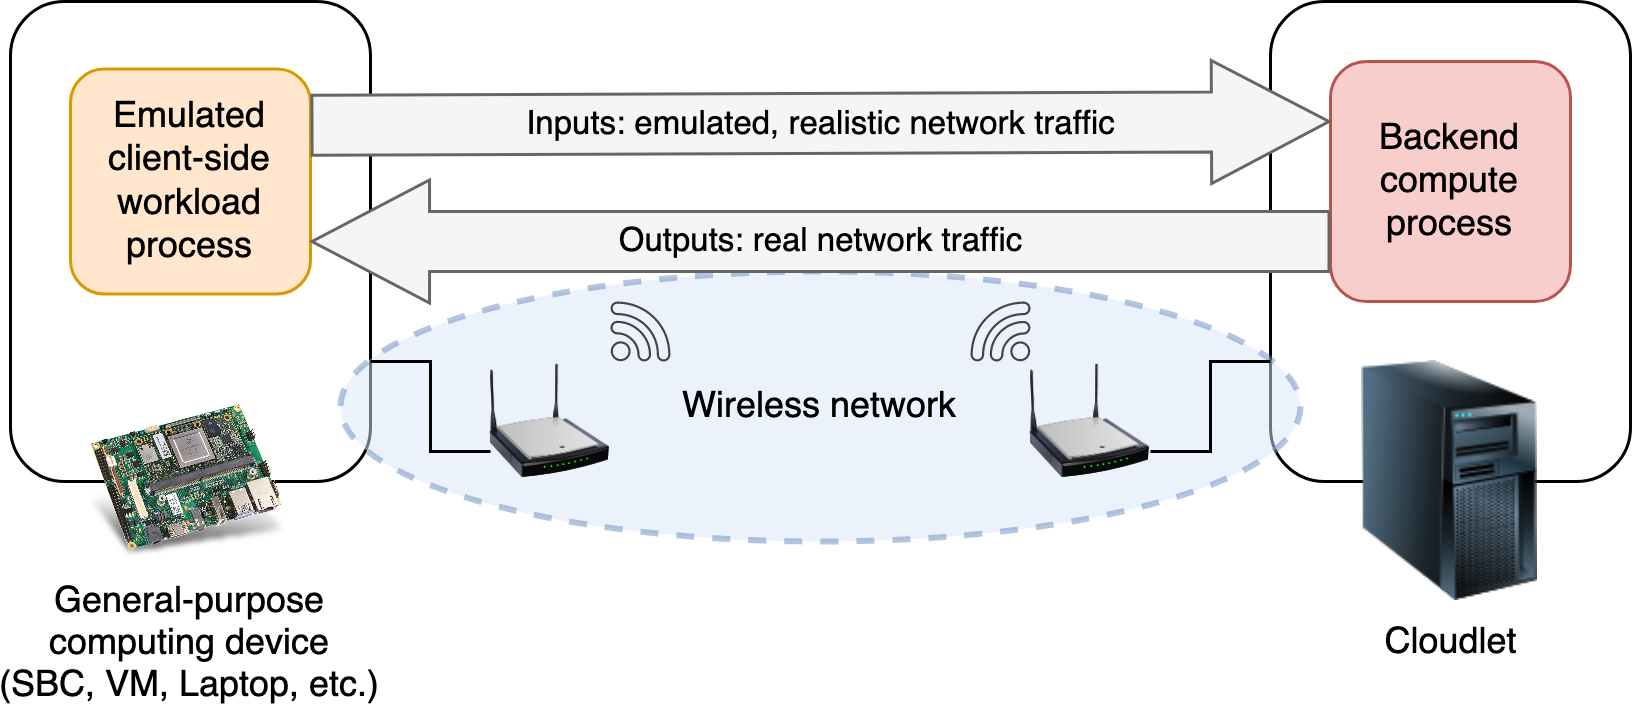
\includegraphics[width=.8\textwidth]{Figs/methodology}
    \caption{%
        Overview of the proposed methodology for the study of latency-sensitive systems on Edge computing infrastructure.
        The  client side of the system is replaced with an emulation executed on a general-purpose computing device.
        The backend/server side of the system along with the network remain unchanged.
    }\label{fig:methodology}
\end{figure}

Our methodology is based on the emulation of target workloads on actual Edge infrastructure;
see \cref{fig:methodology}.
We replace the client side of the system with a realistic emulation of the desired behaviors;
this emulation is implemented in software deployed on \gls{COTS} general-purpose computing devices.
In our initial implementation, these correspond to low-cost, easily replaceable and scalable Raspberry Pi 4 Model B~\cite{raspberrypi} \glspl{SBC}.
We aim to maintain the backend software and hardware, as well as the network, unchanged with respect to the real-world deployment, in order to preserve as much realism as possible in the effects arising from the hardware and network.

% As discussed in \cref{chap:relatedwork}, most research in this field falls into either simulated or fully-practical real-world approaches.
Our emulated methodology presents several advantages over alternatives, simulated or fully-practical approaches.
To begin with, and perhaps most importantly, it makes our approach portable and applicable to real Edge computing deployments.
By limiting the emulation to the workload, our approach can be directly employed on pre-existing Edge computing infrastructure in order to benchmark applications before they are deployed.
This makes our approach valuable to not only to the research community, but also to system designers and application developers.

In hand with the previous point, it allows for easier scaling compared to real-world studies.
The systems we target exhibit a centralized nature in which a potentially large number of clients offload computation to a single central compute node.
The client-side component of the applications of interest for this research is often complex to scale.
Consider a system owner interested in studying the performance of some Edge computing setup for latency-sensitive applications.
In the case of interactive and immersive applications, scaling the number of human users is a significant challenge, as recruiting participants is an expensive and time-consuming endeavor.
Scaling applications involving \glspl{CPS} such as \glspl{NCS} can be prohibitively complex and expensive depending on the specific hardware involved.
In many cases, these systems are made-to-order, further increasing the cost as economies of scale cannot be employed.
On the other hand, a simulated approach requires modeling not only the application workload, but also the Edge computing system and infrastructure.
Due to the intricate nature of contemporary cloud and Edge computing setups, which frequently involve multiple tiers of proxies, load balancers, virtualized computing units, and network functions, the modeling of such systems can quickly become an overly complex endeavor.

Our approach circumvents both of these limitations.
Emulating the workload component reduces complexity by moving it into the software domain, allowing for easier scaling through the use of cheap, \gls{COTS} general-purpose hardware such as the aforementioned \glspl{SBC}.
Furthermore, it preserves the realism of effects stemming from the hardware and network.
Employing emulations allows our methodology to realize a more realistic testing environment than a simulated approach and can provide results that are closer to what would be seen in the real-world.
Of particular interest to us are effects due to network factors such as contention, congestion control, and medium access.
These effects are often of stochastic or chaotic natures, and are thus complex to capture in simulations.

Emulating the workload also provides improved repeatability and replicability.
Repeating a study becomes a matter of re-running the workload on the same testbed;
in turn, studies can be replicated simply by obtaining the same or equivalent software workload and deploying it on a comparable testbed.
These are complex tasks to accomplish in real-world approaches, particularly when dealing with humans.

Finally, our methodology improves extensibility significantly.
Replicating the methodology for other workloads simply requires developing a new piece of software to emulate the new workload.
This can further be simplified by employing software platforms for the emulation of categories of workloads, as well will discuss later on in this thesis.

\medskip
In the following subsections we will discuss two illustrative case studies for our methodology; \acl{WCA} and \acl{NCS} research and benchmarking.
\Cref{summary:methodology:usecase_wca} discusses the application of our methodology to \gls{WCA}.
This work was originally published in \cref{paper:olguinmunoz2018demoscaling,paper:olguinmunoz2019edgedroid}.
Next, in \cref{summary:methodology:usecase_ncs} we expand this discussion to \glspl{NCS}, a discussion originally approached in \cref{paper:olguinmunoz2022cleave}.

\subsection{Case study: \acl{WCA}}\label{summary:methodology:usecase_wca}

We first introduce our methodology and its applicability to \gls{WCA} in \cref{paper:olguinmunoz2018demoscaling,paper:olguinmunoz2019edgedroid}.
The former corresponds to an extended abstract paper which discusses a high level overview of our approach;
the latter presents a deeper, more complete discussion about the implementation together with some first experimental results.
As discussed in \cref{chap:introduction,sec:relwork:xremulation}, the main challenge to benchmarking \gls{WCA} --- and other ``human-in-the-loop'' applications on the Edge --- concerns the involvement of human beings in their operation.
Humans are unreliable, and, perhaps more importantly, hard to scale.

The implementation of the client-side emulation necessary for our methodology follows in these works a trace-based design.
The trace-based approach is chosen for three reasons:
\begin{inlineenum}
    \item realism in terms of payloads sent over the network
    \item simplicity without complex modeling of human behavior
    \item extensibility through the recording of new traces for different tasks in the same category of WCA applications
\end{inlineenum}.
This approach provides a realistic execution path while being easily obtainable through instrumentation of existing WCA client applications and easily extensible to different tasks.

While a trace-based emulation approach has advantages in providing realistic inputs without complex modeling of human behavior, it can have a significant drawback:
if system responsiveness at trace replay time differs from system responsiveness at trace recording time, the trace can very easily end up out-of-sync.
To address this, the concept of a user model is introduced, which adapts the replay of the trace to the responsiveness of the system by making slight modifications at runtime.
The user model attempts to navigate the task model and reach the desired system state in light of changing system conditions, while still using the original trace as the source of input data.

\begin{figure}
    \centering
    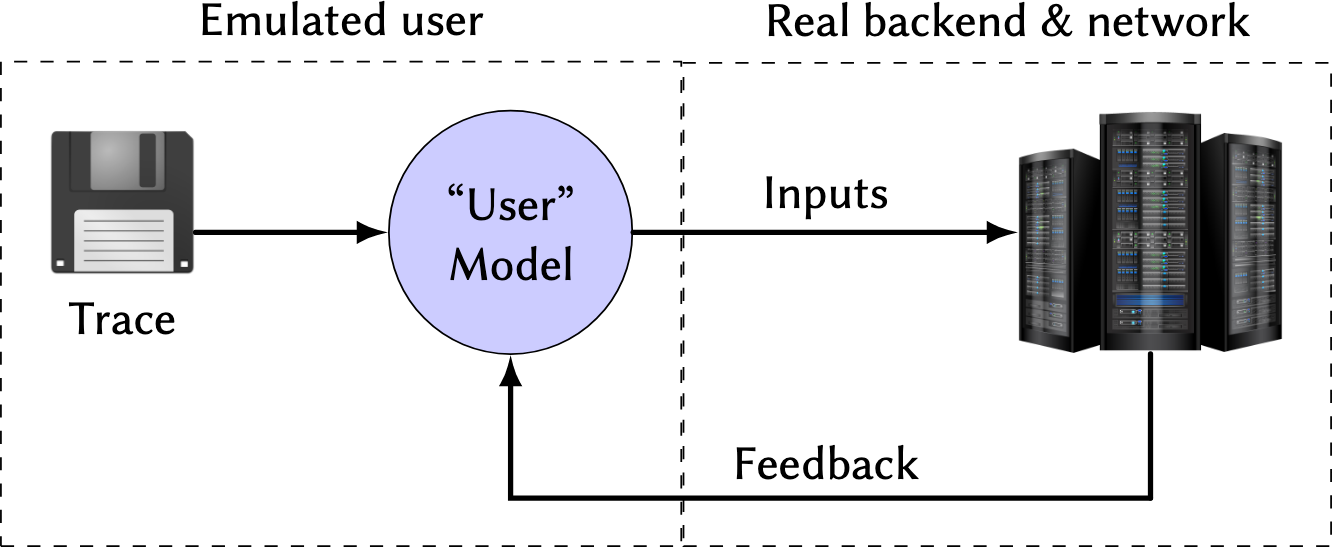
\includegraphics[width=.9\textwidth]{Figs/trace_edgedroid}
    \caption{%
        High level conceptual design of our methodology for \gls{WCA}.
        We replace the human by a trace-driven emulation.
        This allows us to maintain realism in inputs sent over the network to the compute process on the backend, while simplifying the design of the client software.
%        Figure originally published in \cref{paper:olguinmunoz2018demoscaling,paper:olguinmunoz2019edgedroid}.
    }\label{fig:methodology:wca:conceptual}
\end{figure}

\Cref{fig:methodology:wca:conceptual} presents a conceptual diagram of this approach.
The trace is fed to a model of human behavior, which then replays it to the real \gls{WCA} backend.
Feedback from the backend is then interpreted by the model to adapt the runtime replay of the trace.

We introduce a tool, \emph{EdgeDroid \num{1.0}}, which implements the concepts outlined above.
The tool is implemented in Android, allowing for its easy deployment on the same kind of \gls{COTS} mobile and/or wearable devices (e.g.\ Google Glass~\cite{googleglass}) on which real \gls{WCA} applications are intended to run in the future, and is instrumented for easy collection of a multitude of system-level metrics at runtime which can then be analyzed.
We use a trace corresponding to a pre-recorded sequence of sensory inputs obtained from a real execution of the \gls{WCA} by a human volunteer;
the trace is recorded in a near-ideal setting, such that it does not include either human mistakes or segments with degraded system responsiveness.
Finally, we employ in this work a preliminary model of human behavior which is totally impervious to poor system performance, and suffers no annoyance, fatigue, frustration, nausea or other shortcomings of real human users.
This leads to a model of an ``ideal'' user who responds in a precisely reproducible and deterministic manner to the same system stimulus every time.

\medskip
We proceed to demonstrate the practical utility of our methodology as applied to \gls{WCA} by setting up a series of scenarios.
We deployed a \emph{Gabriel}-powered~\cite{chen2018application} \gls{WCA} application on a small testbed consisting of
\begin{inlineenum}
    \item a server computer acting as a cloudlet
    \item a 802.11n Wi-Fi \gls{AP} connected to the cloudlet via ethernet
    \item \num{10} Android smartphones connected wirelessly to the \gls{AP}, emulating users for the application
\end{inlineenum}.
Three scenarios were considered, corresponding to setups under ideal network conditions with \num{1} and \num{10} clients, plus an additional scenario with \num{10} clients located at a distance from the \gls{AP} such that the signal strength was significantly degraded.
Each scenario was repeated a \num{100} times for statistical validity.

\begin{figure}
    \begin{subfigure}[t]{.45\textwidth}
        \centering%
        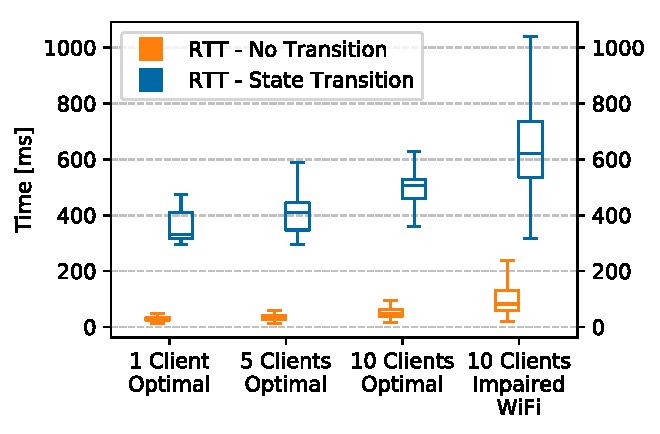
\includegraphics[width=\textwidth]{publications/2019EdgeDroid/plots/comparison/nofonts/rtt_fb_vs_nofb}%
        \caption{
            Comparison of round-trip-times for inputs that triggered a state transition in the task model versus inputs that did not.
        }\label{fig:wca:rtt}%
    \end{subfigure}%
    \hfill%
    \begin{subfigure}[t]{.45\textwidth}
        \centering%
        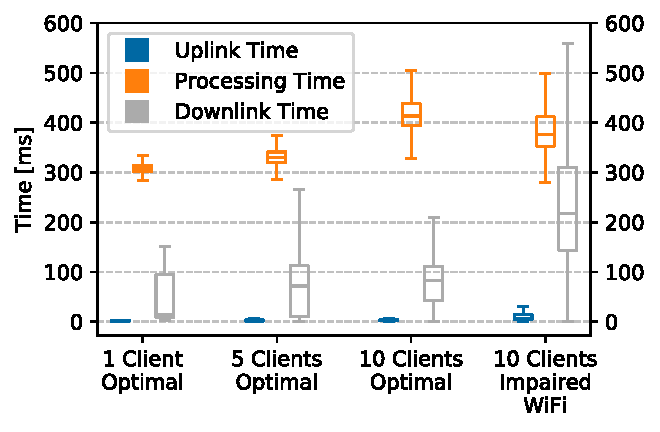
\includegraphics[width=\textwidth]{publications/2019EdgeDroid/plots/comparison/nofonts/box_feedback}%
        \caption{%
            Distribution of latency across system components for inputs that triggered a state transition in the task model.
        }\label{fig:wca:latency}
    \end{subfigure}%
    \caption{
        Example results from the \acs{WCA} case study.
        Figures originally published in \cref{paper:olguinmunoz2019edgedroid}.
    }
\end{figure}

These setups already showcase the flexibility of our approach.
Our trace-based implementation of the methodology allows for detailed measurements of system performance at different levels, from individual components to specific task steps.
This provides valuable insights into the bottlenecks and areas for optimization in the system.
We find, for example, that \glspl{RTT} for feedback-rich inputs are up to an order of magnitude greater than feedback-less inputs\footnote{%
    In this context, \emph{feedback-rich} inputs refer to inputs which trigger a transition in step in the internal task model of the application and thus cause the generation of feedback which is then provided to the user.
    Conversely, \emph{feedback-less} inputs are inputs which are silently discarded at the backend and do not generated noticeable feedback.
}; see \cref{fig:wca:rtt}.
The flexibility of the methodology also allows researchers to zoom into specific components or steps of the system to gain deeper insights, which can inform the design and development of future systems.
For example, the results in \cref{fig:wca:latency} suggest that improving the quality of the wireless link should be a priority for scaling the application.
The system scales linearly with respect to the number of clients, but the impaired Wi-Fi greatly affects the performance of feedback-rich inputs, with delays sometimes exceeding the threshold for acceptable user experience.

Overall, the study demonstrates the usefulness of the trace-based methodology in evaluating system performance.
The results also underscore the need for optimization of system components and the importance of network quality in delivering a satisfactory user experience.

\subsection{Case study: \acsp{NCS}}\label{summary:methodology:usecase_ncs}

We discuss an initial case study of our methodology in the context of \glspl{NCS} and similar \glspl{CPS} in \cref{paper:olguinmunoz2022cleave}.
In this work, we present \gls{CLEAVE}, a software-based framework for scalable and repeatable benchmarking of Edge-native \aclp{NCS}.
The growing adoption of Edge computing has made it important to understand the strengths and weaknesses of different Edge concepts for the deployment of such \glspl{CPS}.

\gls{CLEAVE} is a fully virtualized benchmarking framework, inspired by our previous work in \cref{paper:olguinmunoz2018demoscaling,paper:olguinmunoz2019edgedroid} on benchmarking human-in-the-loop applications on the Edge.
In the case of \gls{CLEAVE} however, we forgo the trace-based approach of EdgeDroid in favor of direct modeling of the target systems.
\gls{CLEAVE} includes a benchmarking framework and software development kit for the development of emulated physical systems and softwarized controllers.
These virtual \glspl{CPS} can then be deployed on real networks for reparametrizable, repeatable, and reproducible benchmarking.

\gls{CLEAVE} is built using Python 3.8, making it highly extensible and able to use existing libraries.
It is compatible with container technologies such as Docker~\cite{docker}, making it suitable for automated deployment, scaling, and benchmarking on industry-standard Edge setups using container orchestration solutions.

\begin{figure}
    \centering
    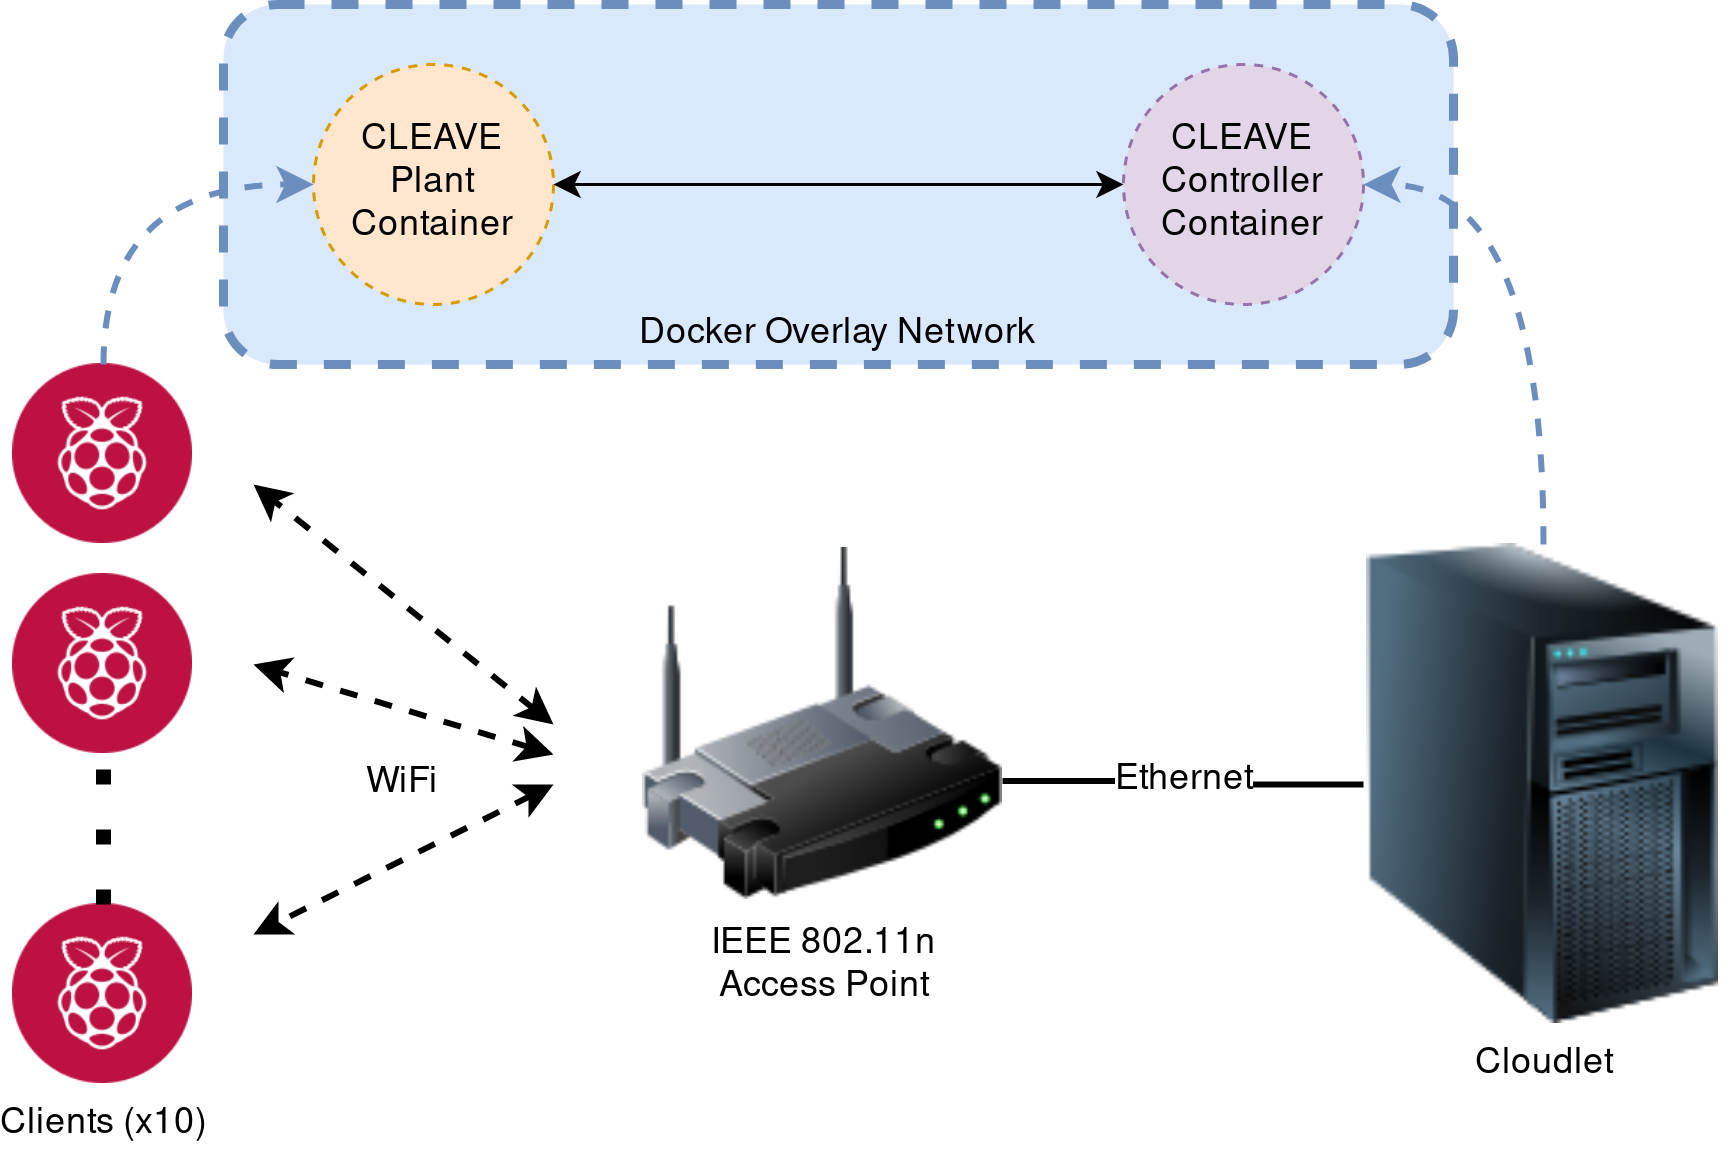
\includegraphics[width=.9\textwidth]{publications/2022CLEAVE/images/CLEAVE_experiment_setup}
    \caption{
        The setup used for experimentation in the \gls{NCS} case study.
        Figure originally published in \cref{paper:olguinmunoz2022cleave}.
    }\label{fig:cleavesetup}
\end{figure}

\medskip
We study the validity of our methodology and the implementation of the software framework through a simple scenario, illustrated in \cref{fig:cleavesetup}.
An inverted pendulum plant controlled by a proportional-differential controller is deployed on an Edge server over a Wi-Fi link, while video-streaming applications run concurrently on the setup.
The inverted pendulum is a popular benchmark in control-system literature, and the setup allows for straightforward reparametrization and a broad range of experiments.
Video analytics, on the other hand, is a main proposed use case for Edge computing, and it is likely that Edge \gls{NCS} deployments will be deployed in parallel with such applications in the future.
Using Wi-Fi allows for more experimental freedom, as the system can be adapted to study both best-case and worst-case scenarios with low and high latencies, respectively.

We first establish a baseline by deploying a single control loop.
This setup is repeated multiple times with different sampling rates to obtain statistically significant results.
The results of the single-loop scenarios show, as expected, that higher sampling rates tend to correlate with better quality of control and that network delays can be compensated for by increasing the sampling rate.

\begin{figure}[t]
    \centering
    \begin{subfigure}[t]{.45\textwidth}
        \centering
        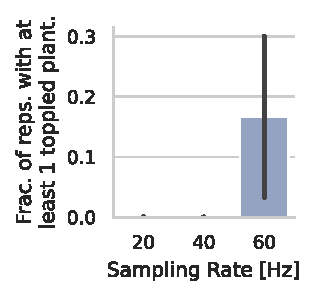
\includegraphics[width=\textwidth]{publications/2022CLEAVE/plots/fixed_video_topple_frac}
        \caption{Fraction of experimental runs with at least one toppled plant.}%\label{paper:olguinmunoz2022cleave:fig:video:toppled}
    \end{subfigure}%
    \hfill%
    \begin{subfigure}[t]{.45\textwidth}
        \centering
        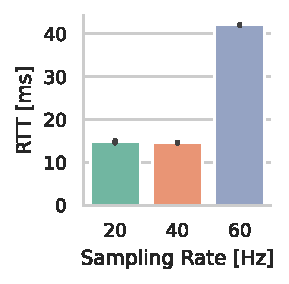
\includegraphics[width=\textwidth]{publications/2022CLEAVE/plots/fixed_video_rtt}
        \caption{\glspl{RTT}.}%\label{paper:olguinmunoz2022cleave:fig:video:rtt}
    \end{subfigure}%
    \caption{
        Results from experimentation with multiple \gls{CLEAVE} control loops co-deployed with video streaming applications.
        Error bars indicate \SI{95}{\percent} \glspl{CI} in all plots.
        Figures originally published in \cref{paper:olguinmunoz2022cleave}.
    }\label{fig:cleaveresults}
\end{figure}

Next, we study the interaction between the control systems and the video-streaming applications.
Six control loops are deployed, as uplink \gls{UDP} traffic from four clients is generated to emulate the load generated by Full-HD video streaming.
Based on the baseline results, we execute scenarios with varying plant sampling rates and repeat each scenario \num{30} times.
Representative results from this experimentation are showcased in \cref{fig:cleaveresults}.
While the baselines might lead us to think that higher sampling rates are always better for the stability of control systems, the results from these experiments show that network and resource contention are important factors when designing \glspl{NCS} for deployment on the Edge.
As sampling rates increase, a critical point is eventually reached at which the congestion on the network link is such that it severely impacts the quality of control.
We conclude that adaptive sampling might be thus a viable method for optimizing resource utilization in these systems.

The results of the experiments will be useful for optimizing resource utilization in Edge-bound networked control systems.
The results of the experiments with video-streaming applications will add to the understanding of the interaction between control systems and networked applications.
Furthermore, the success of our experimentation shows that our methodology, implemented through \gls{CLEAVE}, makes the repeated experimentation and data collection convenient compared to fully physical setups, while at the same time providing enhanced realism with respect to simulated approaches.

\subsection{ExPECA Testbed \& the Ainur software stack}\label{sec:testbed}

After our initial implementation and experimentation with our methodology for \gls{WCA} applications, we realized that creating a testbed for experimental Edge Computing research for would significantly enhance our work.
Establishing such testbed would provide a dedicated and controlled environment that can accelerate future research by eliminating the need for ad-hoc implementations for each new study.
Moreover, having a standardized baseline would make it easier to compare results across different studies.
The testbed could serve as a platform for researchers to test new ideas and compare them to the results of previous experiments.
This would enable more efficient and accurate assessments of the methodology's performance and facilitate the development of new methods and techniques.
Additionally, by establishing a testbed, we could provide a platform for other researchers within our group to conduct their research and experiments.

These reasons led to the establishment of the \gls{EXPECA} testbed at \pgls{KTH}.
\gls{EXPECA} is a \gls{SSF}-funded infrastructure project targeting the development and provisioning of an Edge computing infrastructure for research into novel applications and network architectures.
It consists of a cluster of hardware-reconfigurable \gls{COTS} computing nodes interconnected using managed switches and \glspl{SDR}.
This allows us to quickly, on-the-fly, and in an automated fashion change the characteristics of the cluster and the network, in order to study different Edge- and Cloud-computing deployments and the applications that run on them.

\begin{figure}
    \centering
    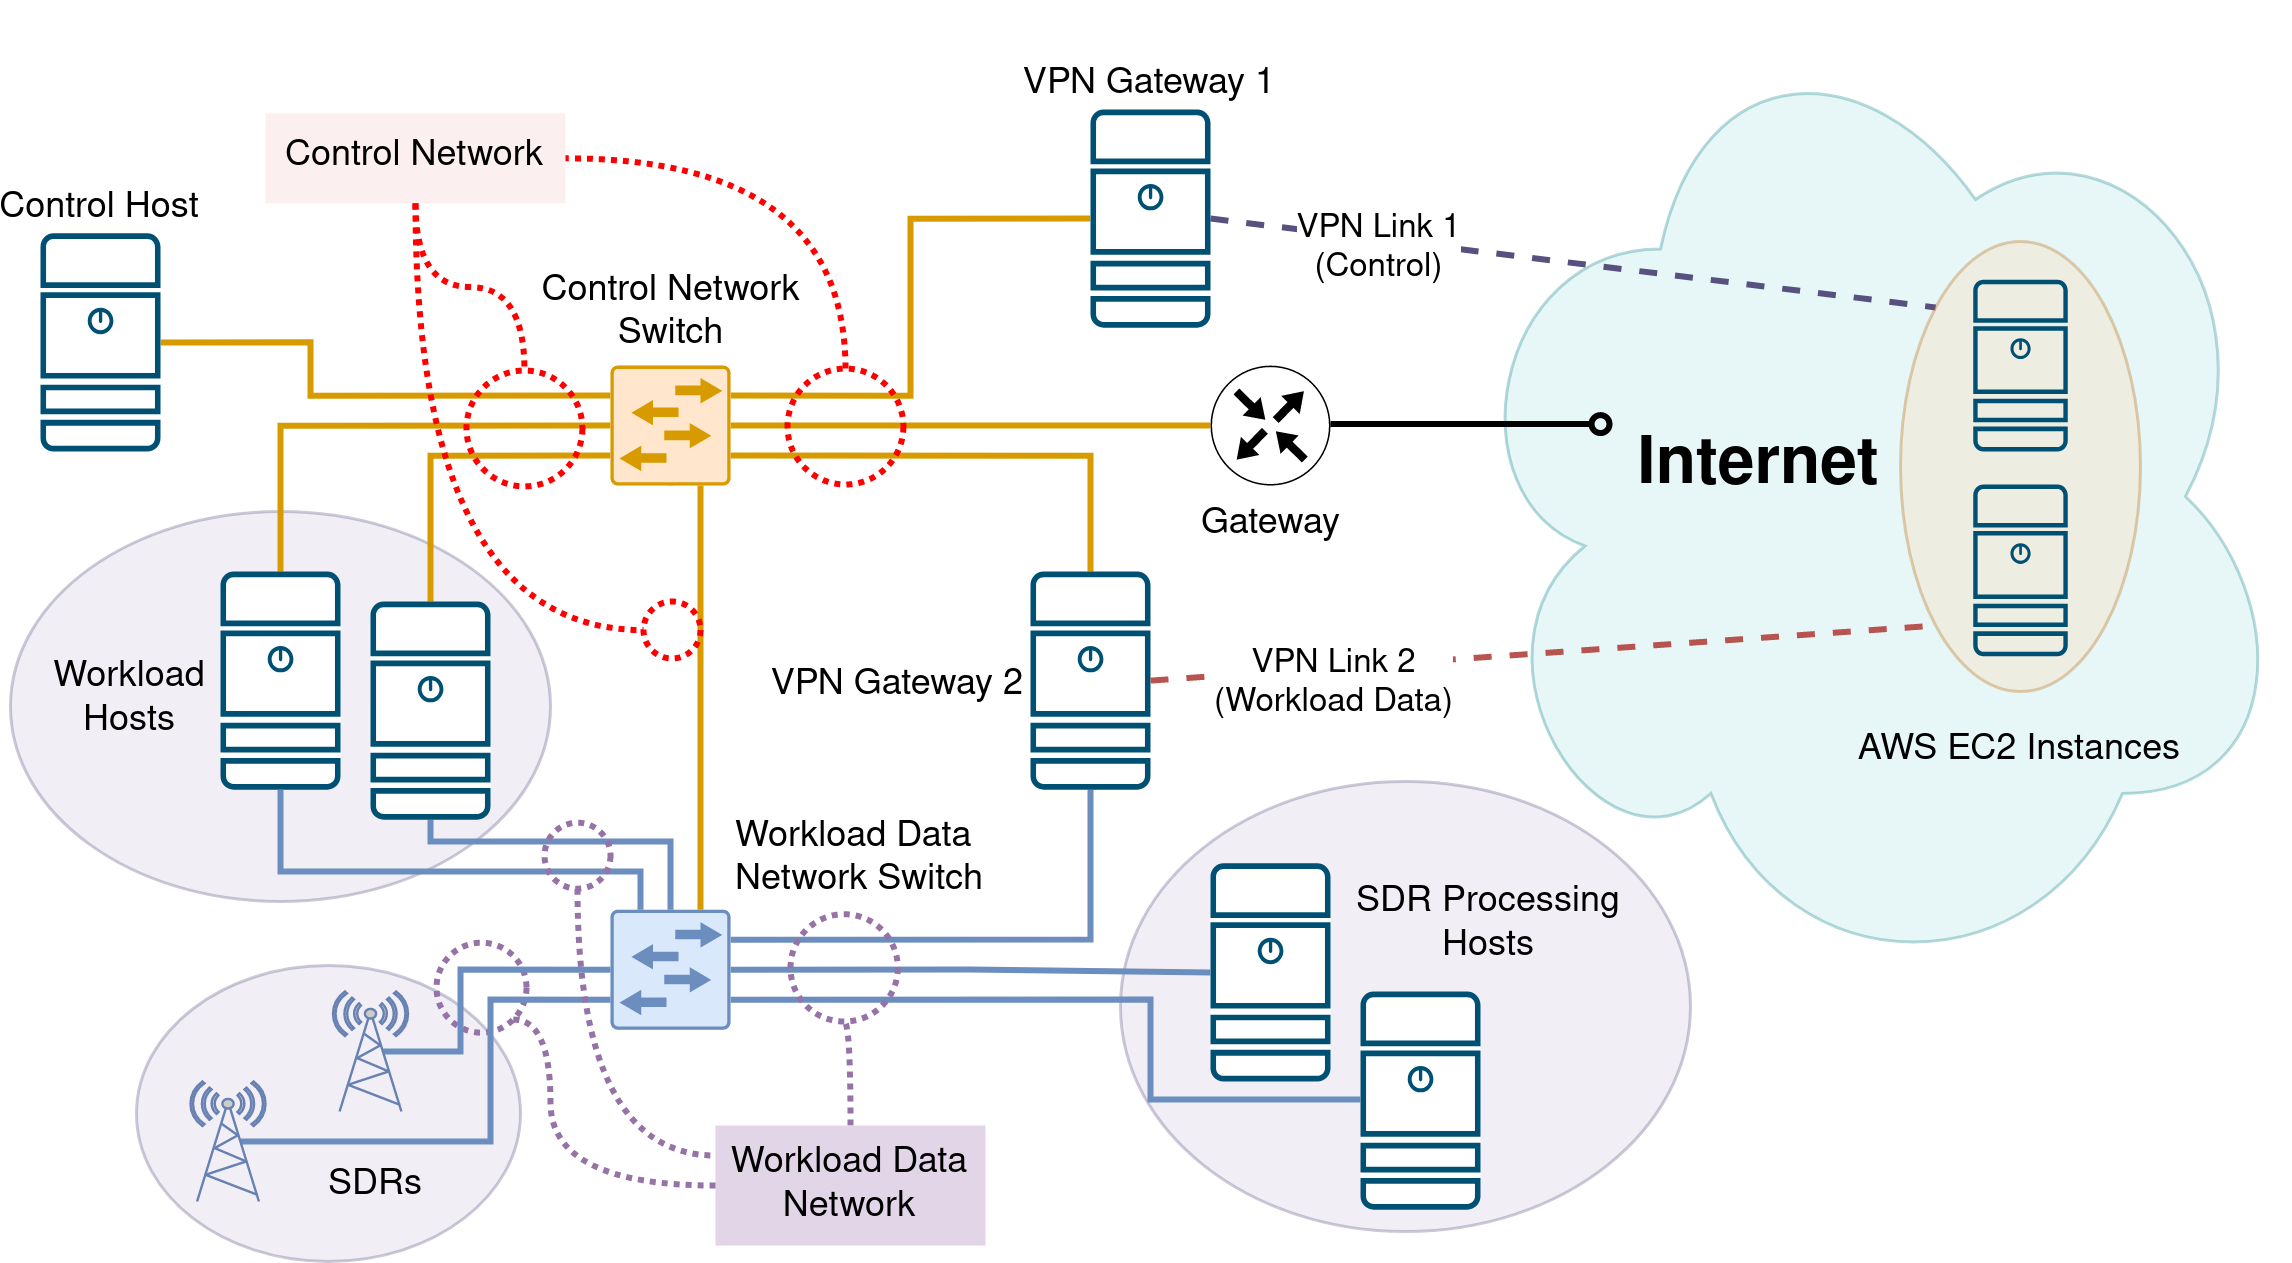
\includegraphics[width=.9\textwidth]{publications/2022Ainur/figures/network}
    \caption{
        Prototype architecture of \acs{EXPECA}.
        Figure originally published in \cref{paper:olguinmunoz2022ainur}.
    }\label{fig:expeca}
\end{figure}

The initial prototype architecture of \gls{EXPECA} is illustrated in \cref{fig:expeca}.
\emph{Workload hosts} act as client-side user devices;
in our prototype, these corresponded to \num{10} Raspberry Pi 4 Model B boards.
These devices connect to either a cloudlet or cloud computing instances over the \emph{workload data network}.
Through clever configuration of \acsp{VLAN} and routing, traffic on this network can be forced to flow through the attached \acsp{SDR} and their associated radio processing hosts.
This allows us to seamlessly switch out the physical layer for experiments.
We implemented configurations wherein one of the \glspl{SDR} acted as a 4G or 5G base station and the other one as a cellular client.
An alternative setup had the workload hosts connect wirelessly via Wi-Fi to one of the radios acting as an \gls{AP}
Finally, the \emph{control network} is used for the out-of-band configuration of testbed resources, and the \acs{VPN} links allow direct tunneled connections to cloud compute nodes on \acs{AWS}.

We also introduce a software framework we developed for its automation and experiment orchestration, \emph{Ainur}.
Ainur is a highly flexible end-to-end wireless network testbed management framework.
Its objective is to facilitate the study of the effects of communication and computation elements on the performance of distributed applications.
To achieve this, Ainur provides a Python \gls{API} that allows researchers to describe experiments in a procedural manner, with plans to eventually offer toolkits for declarative configuration.

The architecture of Ainur closely resembles the conceptual layers of the \acs{TCP}/\acs{IP} stack, and the framework utilizes containerization throughout.
This includes the deployment and orchestration of workloads, support for different physical layer configurations, and automated collection of logs.
To support this, the framework leverages Docker Swarm~\cite{docker,merkel2014docker,Swarm2021} as the container orchestration layer.
Docker Swarm was chosen for its lightweight nature, simple configuration, and inclusion in the default Docker runtime installation.
This allows Ainur to remain agnostic to the nature of the workloads and support a wide range of applications and system architectures, without having to consider library dependencies.

Ainur also leverages containerization for the communication stack, which can nowadays be deployed on general-purpose processors using \gls{O-RAN} and \glspl{SDR}.
This allows for the distribution of the communication stack across multiple hosts, providing researchers with the ability to study the effects of communication and computation elements on the performance of distributed applications.

Finally, we note that both Ainur and \gls{EXPECA} were utilized for experimentation in \cref{paper:olguinmunoz2022cleave,paper:olguinmunoz2023realistic}.
The use of these tools was, however, during their development and prototyping, and they have thus not been referred to by name in these works.
Their first formal appearance was in \cref{paper:olguinmunoz2022ainur}.
